\documentclass{article}
\usepackage[utf8]{inputenc}
\usepackage{authblk}
\usepackage{graphicx}


\title{Multiphonon: Phonon Density of States tools for Inelastic Neutron Scattering Powder Data}
\author[1]{Jiao Y. Y. Lin \thanks{Corresponding author}}
\author[2]{Max Kresch}
\affil[1]{linjiao@ornl.gov, Neutron Data Analysis and Visualization Division, Oak Ridge National Lab}
\affil[2]{mkresch@gmail.com}

\date{September 2017}

\begin{document}

\maketitle

\section{Summary}\label{summary}

The multiphonon python package calculates a phonon density of states from
inelastic neutron scattering (see, for example \cite{FultzINSbook})
spectrum from a powder sample. The algorithm is a self-consistent,
iterative procedure that finishes when
the measured spectrum can be accounted for by
the one-phonon scattering, multi-phonon scattering, and multiple
scattering from the deduced phonon density of states, under the
incoherent approximation (Appendix of \cite{KreschNickel2007} and
Section 6.5 ``Calculation of Multiphonon Scattering'' of
\cite{FultzINSbook}).

\begin{figure}
  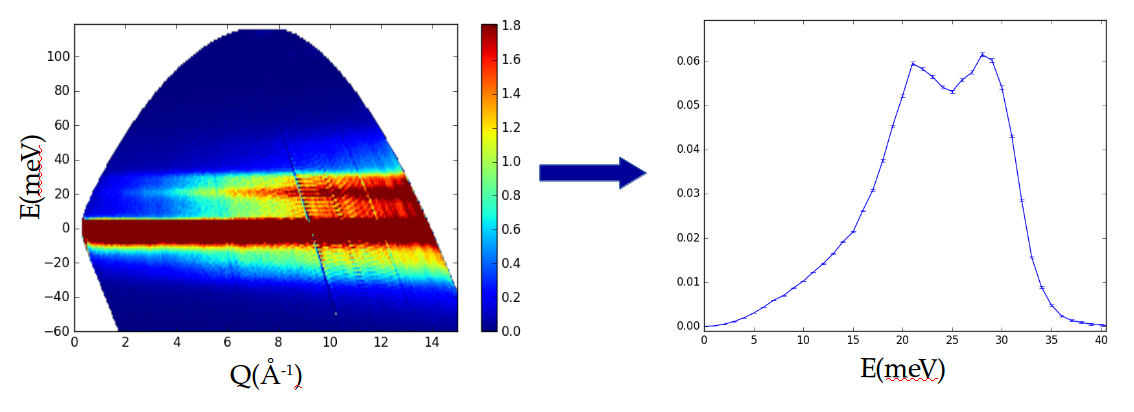
\includegraphics[scale=0.25]{sqe2dos}
  \caption{The multiphonon package takes the inelastic neutron scattering spectrum, shown on the left, and produces the phonon density of states shown on the right.}
\end{figure}


\section{Notice of Copyright}\label{notice-of-copyright}

This manuscript has been authored by UT-Battelle, LLC under Contract No.
DE-AC05-00OR22725 with the U.S. Department of Energy. The United States
Government retains and the publisher, by accepting the article for
publication, acknowledges that the United States Government retains a
non-exclusive, paid-up, irrevocable, worldwide license to publish or
reproduce the published form of this manuscript, or allow others to do
so, for United States Government purposes. The Department of Energy will
provide public access to these results of federally sponsored research
in accordance with the DOE Public Access Plan
(http://energy.gov/downloads/doe-public-access-plan).

\section{Acknowledgements}\label{acknowledgements}
This work is sponsored by the Laboratory Directed Research and
Development Program of Oak Ridge National Laboratory, managed by
UT-Battelle LLC, for DOE. Part of this research is supported by the U.S.
Department of Energy, Office of Science, Office of Basic Energy
Sciences, User Facilities under contract number DE-AC05-00OR22725.
We thank Douglas Abernathy, Jennifer Niedziela, Iyad Al-Qasir, 
Dipanshu Bansal, and Chen Li for stimulating discussions.


\bibliographystyle{unsrt}
\bibliography{paper}

\end{document}
